\chapter{Current System Or Situation \\
%\small{\textit{-- Team-11}} 
\index{Chapter!Current System Or Situation }
\index{Scope}
\label{Chapter::Current System Or Situation}}
The motivation behind developing this system is that currently, stakeholders, which in this case would be common person, without much knowledge about the law, are required to manually read through terms and conditions contracts which can often be super long, time consuming and notoriously confusing due to the amount and complexity of the legal terms used, that are at the end of the day, accepted in a court of law, which would be unfamiliar to a common person thereby, risking themselves of inflicting harm in a shape that may result in financial, personal or mental distress. While the option to consult a lawyer exists, it is not always feasible due to their high costs and availability constraints.

In the absence of an effective tool to navigate this challenging problem, the need for a solution like ClauseGuard became apparent. This system is designed to safeguard stakeholders from potential pitfalls hidden in deceptive clauses. By providing a machine learning-based analysis of contracts, ClauseGuard offers a reliable, user-friendly, and cost-effective alternative to traditional methods of consulting a lawyer, fostering a safer and more transparent contract review process.  

\section{Background, objectives, and scope \label{Section::Background,objectives and scope} }
The current system exists to ensure that stakeholders, typically common individuals, are equipped to agree to the terms and conditions contracts set forth by the initiating party. This process, however, is often lengthy, complex, time-consuming, and challenging for the average person to fully understand the implications of the contract. While professional consultation is an option, the high costs associated with it often render it an unfeasible choice.

The mission of the proposed system, Clauseguard, is to ensure that stakeholders can effectively parse through the terms and conditions contract presented by the initiating party. The ultimate aim is to make stakeholders aware of any deceptive or harmful clauses in the contract, thereby safeguarding them from potential financial, personal, or other forms of harm.
 The scope of the proposed system extends to stakeholders from any background ranging from a common person to a lawyer, govermental agencies and mega corporations who may encounter contractual agreements. The objective is to provide support and enhance their understanding of the contracts they engage with, regardless of the complexity of the legal language involved. 



% The primary purpose of this project is to protect stakeholders from falling victim to deceptive clauses in contracts that may undermine their best interests, either intentionally or unintentionally or via other disruptive means. These clauses could cause harm to the signing party through various means, such as monetary loss or other negative consequences that may impact the livelihood of the concerned stakeholder as a whole. The proposed machine learning software system aims to detect and flag such fraudulent clauses in terms and conditions contracts, thus empowering stakeholders to make informed decisions before committing to an agreement.

% By leveraging advanced machine learning algorithms, the system will analyze and identify potential risks in the contract language. This approach ensures that stakeholders are aware of any hidden or obscure terms that could be detrimental to their interests. In addition to enhancing the transparency of contractual agreements upheld in a court of law, the software will enable users to negotiate better terms, minimize potential disputes, and ultimately establish a more secure and trustworthy contractual environment.

\section { Operational policies and constraints \label{Section::Operational Policies and constraints}}
There are a number of operational policies and constraints that are applied to the proposed system.
\subsection{Operational Policies}
An operational policy can be defined as a general statement of required behaviour. The operational policy of clauseguard is as follows: 
\begin{itemize}
    \item Data privacy is a major cause of concern for the proposed system. Sensitive and confidential information would be shared on an open internet website. As such, the system must ensure that no information is stored on any backend servers in the form of "cookies", "tokens" or any similar data logging services. The system should respect data privacy laws partaining to each individual country and follow guidelines as set forth by that particular country. 
    
    \item The system must explicitly ask stakeholders for their consent for analyzing the submitted documents before using the system. This consent would be devised by a team of professional experts and lawyers so as to not hold the parent organization of clauseguard of any legal ramifications. 

    \item The system must utilize a sophisticated machine learning algorithm that is retrained and updated at intervals of every two months. This ensures that the model stays current with the evolving nature of legal language in contracts, reflecting the latest laws and regulations. Additionally, cross-checking with historical legal data is done during these updates to maintain consistency and accuracy. Periodic reviews by legal experts complement the machine learning model, ensuring its recommendations remain accurate and legally sound.

    \item the system must provide clear explanations for any detected clauses in the Terms & Conditions contracts. These explanations are devised by the system based on the analysis of datasets comprising other legal documents of similar nature and scope. This ensures that users not only receive information about potential issues in the contracts they're reviewing, but also gain an understanding of why these clauses may be problematic.
\end{itemize}

\subsection{Operational Constraints}
An operational constraint is an externally imposed condition that must be observed. The operational constraint of clauseguard is as follows: 
\begin{itemize}
    \item The machine learning algrothim would require extreme amounts of processing power and computational resources, which, on failing to secure, would severely limit the number of contracts that can be analyzed. It can also lead to network wide crashes and instability. 
    \item The model depends on the accuracy of the dataset on which it is trained. Lack of available legal documents can induce severe challenge on the authenticity and accuracy of the model. Some countries do not disclose legal documents into the public domain, thereby severely limiting the use of this model in certain geographic locations. 
    \item The model must be online 24/7 365 days of the week. Lack of server resources can cause an availability constraint. 
    \item The model must comply with data regulations  and privacy laws around the world. This constraint cannot be guranteed across every country, as each country has extremely wide definations of data privacy laws, failing to adhere can cause a ban of this sytem in that particular country. 
    \item The model must handle contracts written in different terminologies and structures used across various different countries. For example, Japanese legal system requires legal documents to start from the right to left. Training the model on many different structures is a significant operational constraint. 
    \item The model must ensure the security of private and sensitive data. This is also a major operational constraint as unethical hacking can lead to significant data leaks. 
    
\end{itemize}

\section{Description of the current system or situation \label{Section::Description of the current system or situation}}
The current system is being built with the primary objective of developing a machine learning model to aid stakeholders in identifying potentially deceptive clauses in terms and conditions (T\&C) contracts. This system functions by automatically scrutinizing all clauses within the contract, thereby equipping stakeholders with crucial information needed to make an informed decision regarding their agreement to the terms.
The system uses several machine learning libraries such as scikit-learn, natural language toolkit(NLTK) and keras for the creation of the model. 

Scikit-learn is a machine learning library in Python that provides tools for data analysis and modeling. In this system, scikit-learn is primarily used for preprocessing the dataset and training the machine learning model. It provides utilities for common machine learning tasks such as feature extraction, text representation, and model evaluation. For instance, scikit-learn's text feature extraction utilities can convert the text data in T&C contracts into a format that can be input to the machine learning model.
Natural Language Toolkit (NLTK) is a library in Python that provides tools for working with human language data (text).  In this system, NLTK is primarily used for tokenization (i.e. breaking up of sentences into each indidual alphabet, white space, special character, symbol etc), stemming (A process to remove the suffix from words such as ing), and lemmatization (converting the word into its root form and reducing the superlative of the word into its equivalent comparative, for example: oldest will be old), which are crucial steps in preprocessing the text data.

Keras is a high-level neural networks API in Python.  
It is used to define and train any kind of deep learning model. In this system, Keras is used to define the machine learning model structure and train the model using the preprocessed dataset.

Flask and Django are web development frameworks in Python.  In this system, Flask and Django are used to build the web application that allows users to upload T&C contracts and get the results from the machine learning model. Flask can handle simpler and smaller loads, while Django can manage more complex and larger loads. The choice between them would depend on the requirements and scalability plans of the system. Flask would be used for the inital build of the system followed by django for a more advanced model. 

The system operates by facilitating users to upload a T&C contract via a web interface, developed using Flask or Django. The uploaded contract undergoes a preprocessing step, where it's transformed into a suitable format for the machine learning model using libraries such as scikit-learn and NLTK.

The preprocessed data is then fed into a machine learning model, constructed and trained using the Keras library. This model evaluates each clause in the contract, assigning a risk score that represents the likelihood of the clause being deceptive or unfair.

The output provided to the user includes highlighted sections of the contract that have been flagged as potentially deceptive, along with a percentage indicator that quantifies the overall risk associated with the contract. For each highlighted section, the system also provides an explanation, derived from the model's analysis, clarifying why the clause was flagged.

With this information, the user is empowered to make an informed decision about whether to sign the contract or not. 
The breakdown of the system is as follows: 
\begin{itemize}
    \item Operational Environment and its characteristics: The current environemtn invloves stakeholders using a web platform to upload their T\&C contract into a web interface. 
    \item Major system components and the interconnection among those components: The system comprieses of a machine learning model that is trained on a vast amount of datasets invlovling legal documents from various bracnches of the law such as crimaal law, corporate law, copyright protect, patent law, etc. The model parses each line in the contract, signals out protential harmful clauses that may seek to cause harm to the signing party in the shape of montery or mental duress, and quantifies the risk carried with the contract signified by a percentage. Furthermore, the model genewrates expplainations for the harmful clauses it has highlighted. 
    \item Interfaces to external systems or procedures: The system can be accessed on any platform, device and operating systems. Similar to chatgpt, an api for the model will be released whcih can be integrated into propirety systems that are otherwise not avaialbe to the general public and are the intellectual property of their respective owenrs. 
    \item Capabilities, functions, and features of the current system: The system's objective is to analayze and interpret complicated legal terms, identifying potentially harmful clauses and providing layman explainations to the user. The system's function includes parsing throug each line of the document, running the parsed text through the machine learning model and generating a small report accessable within the website itself that includes a risk assessment percentage as well as a succint explaination, 
    \item e)                \begin{figure}[H]
    \centering
    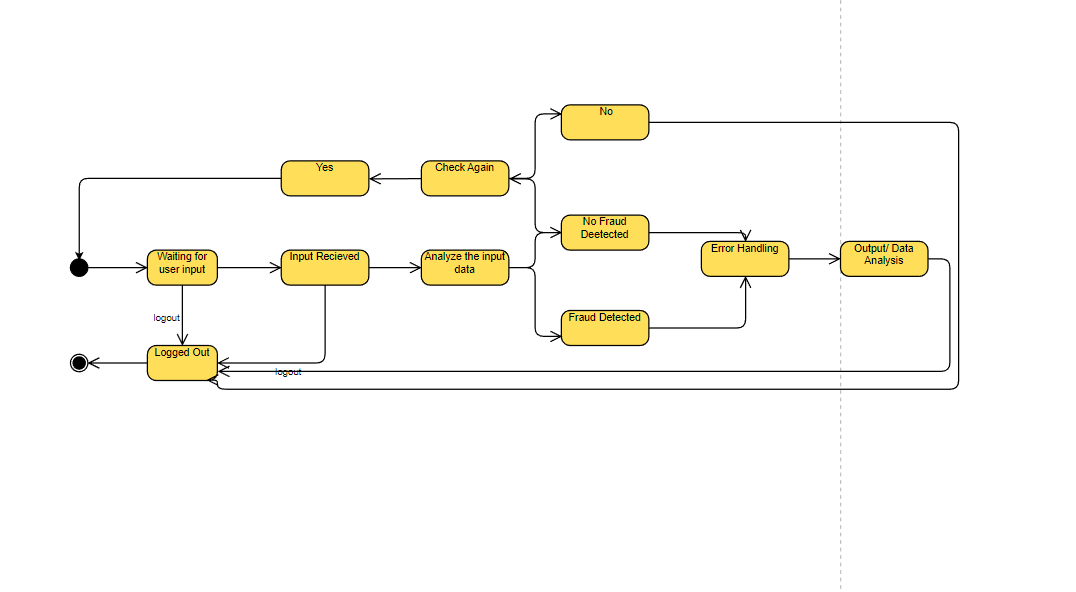
\includegraphics[scale=0.83]{Figures/state machine.png}
    \caption{State Machine View of the diagram \ref{fig:state machine}}
    \label{fig:state machine}
\end{figure}
   

    \item Cost of system operations: The cost of running the system would depend upon the amount of resources that it would take to run the model on servers accessible throughout the world wide web whist analyzing millions of documents concurrently. Load balancers and other such infrastructure must be set up to ensure the working for the model. Infrastructure like the Amazon AWS could be used to set up the model. This would solve the problem with data protection too.  Maintenance would require additional funds. Overall, a cost in the 7 figure range is expected for the initial version of the system 

    \item Operational risk factors: Several operation risk factors could occur which include inaccurate intepretation and explaination, legal reprucssions, confidential Data leaks, Security breaches, server crashes, instability, low accuracy, inaccurate percentages and so on. 
    \item Performance characteristics: The model should be fast, accurate and able to process large quantities of data. To ensure these non-functioanl requirements, the model can be set up on additional infrasture such as could bases services. Amazon AWS would benefit the model tremedously. 
    \item Quality attributes: The model should aim for high availability, reliability and secuity. Becuase of the nature of deleaing with legality of a country, accuracy, avaialbity and reliability are of utomost importance. 
    \item Provisions for safety, security: Due to the nature of the model itself, sensitive and confidential data will be shared. The model must ensure data privacy and secuity of the system to prevent potential breaches and subsequent leaks of confidential data. The system must be designed to ensure high frequency of backed up data to guarantee swift recovery of said data if  operational failures occur. 
\end{itemize}

 



\section{Modes of operation for the current system or situation \label{Section::Modes of Operation for the current system or situation}}
The system will operate on various modes of operation throughout its lifecycle as detailed below: 
\begin{itemize}
    \item Training Mode: This mode is only accessible to the system's developers and not to the end users. It plays a crucial role in the functioning of the system as this is where new features are developed, the model is trained on additional datasets, and existing defects are patched. The training mode uses large amounts of T\&C contracts to train the machine learning model to understand the structure, language, and meaning of various clauses. This process allows the model to learn how to distinguish between benign and deceptive clauses. Enhancements and updates to the system are made in this mode before being deployed to the Operational Mode. 
    \item Operational Mode: This model is the primary end product of the system used by the users to upload T\&C contracts for analysis. The system would use the model developed in the training mode to evaluate the uploaded contract. It identifies potentially deceptive clauses, calculates the overall risk associated with the contract, and provides explanations for flagged sections. The results are then displayed to the user, who can use this information to make an informed decision about whether to sign the contract.
    \item Emergency Mode: This mode serves as a contingency plan, activated in the event that both the Primary and Training modes experience operational failures. The Emergency Mode relies on a legacy version of the currently deployed primary model. This fallback mechanism ensures continuity of service even in the face of unforeseen disruptions. While it may not have the most recent updates and features available in the Primary Mode, the Emergency Mode is designed to effectively analyze T&C contracts and identify deceptive clauses, thereby maintaining the core functionality of the system. Regular checks and minor updates are carried out to ensure that the Emergency Mode is always ready for activation, should the need arise. This robust backup plan contributes to the system's resilience and reliability, offering users a dependable tool for contract analysis at all times.
    


\end{itemize}


\section{User classes and other involved personnel \label{Section::User Classes and other involved personnel}}
Clauseguard would involve the participation several user classes and  personal either directly or indirectly depending upon their interaction with the system as given below: 
\begin{itemize}
    \item End User: The end users are the primary users of clauseguard. They interact directly with the system by uploading the T\&C contracts for analysis. Their interaction is via the web platform, with the aim of identifying deceptive contracts in T\&C contracts. They don't require any skill levels except basic computer skills. 
    \item Developers: They are the primary coders of the system. Their responsibilities include, implementing new features, functionality and maintenance of the system. They require high skill levels in the fields of programming and problem-solving as they require a high level of technical skill and familiarity with the underlying technology.
    \item Machine Learning Specialists: ML specialists work to continually improve clauseguard's machine learning algorithm. They are responsible for training the model on new datasets, testing performance and implementing updates as needed. Their interaction is through machine learning libraries used in the development of the model. 
    \item CyberSecurity Experts: These individuals play a crucial role in safeguarding the ClauseGuard system from unauthorized access and potential security threats and are arguably the most important stakeholders in the functioning of clauseguard as a service. They are tasked with the responsibility of thwarting attempts by unethical entities, often referred to as hackers, who might attempt to breach the system and gain access to confidential data. Cybersecurity experts work diligently to identify and secure any potential vulnerabilities in the system that could be exploited for malicious purposes. Their interaction with the system spans across all areas, but they primarily focus on the system's edge cases and potential weak points that could be susceptible to breaches. They are proficient in the latest cybersecurity protocols and techniques and utilize this expertise to constantly enhance the system's security measures. In addition, they collaborate closely with the system administrators and developers to ensure that security is integrated into all aspects of the ClauseGuard system, from the web application to the machine learning model itself. Their work helps maintain the trust of the end-users by ensuring that their interactions with the system remain secure and confidential.
    \item Legal Consultants: Although their involvement may not be direct, they nevertheless, play a crucial role in the development of the model. They review the machine learning model's output to ensure its accuracy and make recommendations for improvement based on their legal expertise. They interact indirectly with the system by providing feedback and suggestions for model enhancements based on their understanding of legal terminologies and concepts.
    \item Commercial enterprises stand to gain significantly from the use of the ClauseGuard system. These entities often engage in complex transactions that involve extensive legal contracts. With the help of ClauseGuard, they can quickly and efficiently review these contracts, expediting the deal-making process. For instance,  the  purchase of Activision-Blizzard by Microsoft made headlines across the tech industry. In such scenarios, missing or overlooking crucial legal details can lead to considerable impediments, potentially blocking the deal altogether which happened in the case of Microsoft acquiring Activision-Blizzard. ClauseGuard can mitigate such risks by identifying potentially harmful or unclear clauses that could jeopardize the agreement. This can save enterprises substantial time and resources, while also providing them with a layer of protection against contractual pitfalls. Similar to end users, commercial enterprises need only basic computing skills to access clauseguard. 

\end{itemize}


\section{Support environment \label{Section::Support Environment}}
Clauseguard will have a number of support systems in place that will fortify the absolute working of the system to its fullest capacity. 
\begin{itemize}
    \item Clauseguard will have a dedicated technical support team. This team will handle technical queries, troubleshoot reported issues and work on continuous improvement of the system. 
    \item Since clauseguard would primarily be virtual, the equipment and facilities would involve robust server architecture preferbly on cloud bases services such as AWS, load balancers for handling multiple connection requests and IT infrastructure for the support team to handle issues effectively. 
    \item Clauseguard would have a customer service team and infrastructure to manage user inquiries, issues and feedbacks. This platform would involve efficient tracking and resolution of support tickets. 
    \item ClauseGuard , being a cloud-based application, would use secure cloud storage services to store user data and application elements essential for the functioning of the system. It is to be noted that any personal or confidential data will not be stored in any capacity. 
\end{itemize}




